
\begin{center}
	\Huge
	Monotoniforhold og hældninger
\end{center}

\section*{Tangenter og differentialkvotienten}
\stepcounter{section}

Vores næste emne hedder \textit{differentialregning}. Differentialregning omhandler at beskrive vækst og hældninger af \textit{glatte} funktioner - altså funktioner, der ikke har "knæk" og "hop". De fleste funktioner, vi arbejder med i gymnasiet er glatte funktioner - eksempelvis polynomier og eksponentialfunktioner. 

\begin{figure}[H]
	\centering
	\begin{minipage}{0.5\textwidth}
	\centering
	\resizebox{0.9\textwidth}{!}
	{
	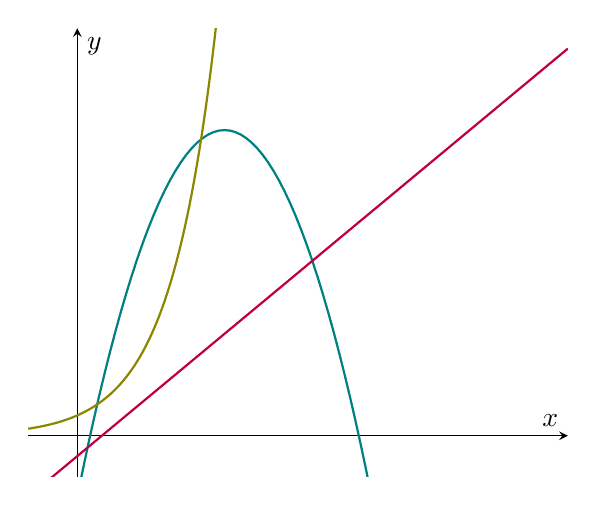
\begin{tikzpicture}
		\begin{axis}[
			axis lines = center,
			xmin = -2, xmax = 20,
			ymin = -2, ymax = 20,
			ticks = none, 
			xlabel = $x$, 
			ylabel = $y$
		]
			\addplot[color = teal, thick, samples = 100, domain = -2:20] {-0.5*x^2+6*x-3};
			\addplot[color = olive, thick, samples = 100, domain = -2:8] {1.7^x};
			\addplot[color = purple, thick, samples = 100, domain = -2:20] {x-1};
		\end{axis}
	\end{tikzpicture}
	}
	\caption{Glatte funktioner.}
	\end{minipage}%
	\begin{minipage}{0.5\textwidth}
	\centering
	\resizebox{0.9\textwidth}{!}
	{
	\begin{tikzpicture}
		\begin{axis}[
			axis lines = center,
			xmin = -2, xmax = 20,
			ymin = -2, ymax = 20,
			ticks = none, 
			xlabel = $x$, 
			ylabel = $y$
		]
			\addplot[color = teal, thick, samples = 100, domain = -2:3] {0.5*x^2+4};
			\addplot[color = teal, thick, samples = 100, domain = 3:20] {-0.5*x + 10};
			\addplot[color = olive, thick, samples = 100, domain = -2:6] {2*x-1};
			\addplot[color = olive, thick, samples = 100, domain = 6:12] {-3*x + 23};
			\filldraw[color = olive] (axis cs: 6,11) circle (2pt);
			\filldraw[color = white] (axis cs: 6, 5) circle (2pt);
			\draw[color = olive] (axis cs: 6, 5) circle (2pt);
		\end{axis}
	\end{tikzpicture}
	}
	\caption{Ikke-glatte funktioner.}
	\end{minipage}
\end{figure}

Hvis en funktion er glat i et punkt - altså at den ikke har nogle knæk eller hop i punktet, siges funktionen at være \textit{differentiabel} i dette punkt. Vi vil senere komme ind på, hvad det helt præcist betyder, men for nu vil det blot være et mere heuristisk begreb. Hvis en funktion er differentiabel i et punkt, kan vi finde differentialkvotienten i punktet. For at definere begrebet differentialkvotient skal vi dog have en fornemmelse for, hvad en tangent til en funktion er.

\newpage
\begin{exa}
	På Figur \ref{fig:tangent} ses grafen for polynomiet $f(x) = x^2$ samt tangenten til grafen i punktet 
	$(2,4)$. 
	\begin{figure}[H]
		\centering
		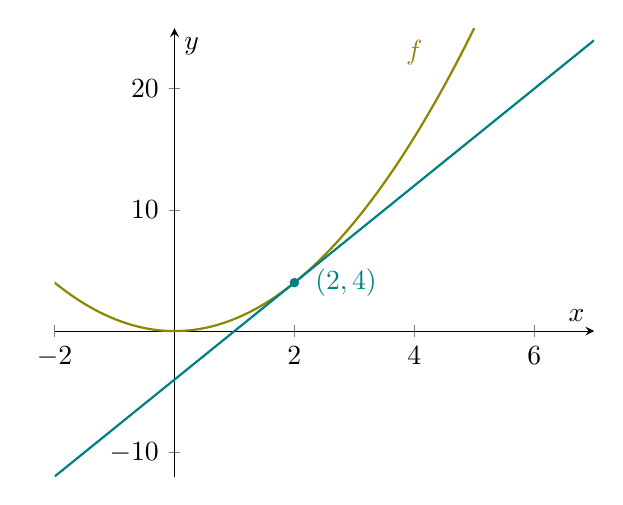
\begin{tikzpicture}
			\begin{axis}
			[
			axis lines = center,
			xmin = -2, xmax = 7,
			xlabel = $x$, ylabel = $y$
			]
				\addplot[thick, color = olive, samples = 100] {x^2};
				\addplot[thick, color = teal, domain = -2:7] {4*x-4}; 
				\filldraw[color = teal] (axis cs: 2,4) circle (1.5pt);
				\node[color = olive] at (axis cs: 4,23) {$f$};
				\node[color = teal, anchor = west, xshift = 4pt] at (axis cs: 2,4) {$(2,4)$};
			\end{axis}
		\end{tikzpicture}
		\caption{Graf for $f$ samt tangent til grafen.}
		\label{fig:tangent}
	\end{figure}	 
	Vi kan se, at tangenten følger langs grafen for $f$ og rører grafen i netop ét punkt; navnligt punktet
	$(2,4)$. Tangenter opfylder den egenskab, at de følger langs grafen og rører grafen for funktion 
	lokalt i netop ét punkt.
\end{exa}
\begin{defn}[Differentialkvotient]
	Differentialkvotienten til en funktion $f$ i et punkt $(x_0,f(x_0))$ defineres som hældningen af tangenten 
	til $f$ i punktet $(x_0,f(x_0))$. Differentialkvotienten betegnes $f'(x_0)$. Hvis 
	differentialkvotienten kan findes for alle $x$, så siges $f$ at være \textit{differentiabel}.
\end{defn}
\begin{exa}
	Betragter vi igen situationen fra Figur \ref{fig:tangent}, så kan vi bestemme hældningen af tangenten til
	$f$ i punktet $(2,4)$ ved aflæsning. Af Figur \ref{fig:tangenttern} aflæses hældningen af tangenten til
	$f'(2) = 4$.
	\begin{figure}[H]
		\centering
		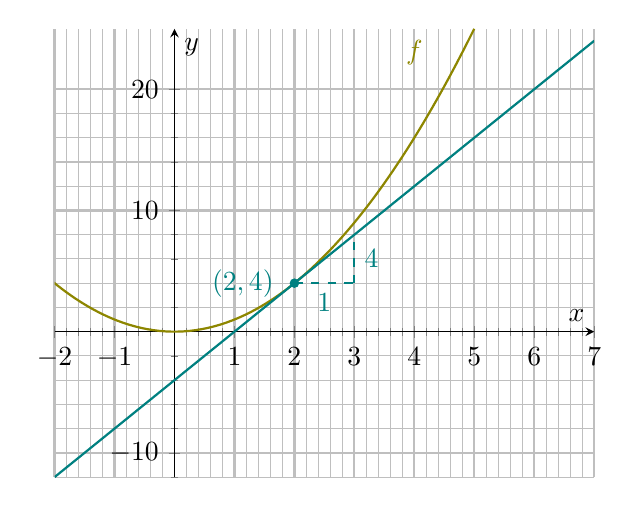
\begin{tikzpicture}
			\begin{axis}
			[
			axis lines = center,
			xmin = -2, xmax = 7,
			xlabel = $x$, ylabel = $y$,
			grid = both,
			major grid style = {line width = 0.8pt},
			xtick = {-2,-1,...,5,6,7},
			minor tick num = 4,
			]
				\addplot[thick, color = olive, samples = 100] {x^2};
				\addplot[thick, color = teal, domain = -2:7] {4*x-4}; 
				\node[color = olive] at (axis cs: 4,23) {$f$};
				\node[color = teal, anchor = east, xshift = -4pt] at (axis cs: 2,4) {$(2,4)$};
				\draw[dashed, thick, color = teal] (axis cs: 2,4) -- (axis cs: 3,4) 
				node[midway, anchor = north] {$1$};
				\draw[dashed, thick, color = teal] (axis cs: 3,4) -- (axis cs: 3,8)
				node[midway, anchor = west] {$4$};				
				\filldraw[color = teal] (axis cs: 2,4) circle (1.5pt);
			\end{axis}
		\end{tikzpicture}
		\caption{Graf for $f$ samt tangent til grafen.}
		\label{fig:tangenttern}
	\end{figure}	 
\end{exa}
\section*{Monotoni}
\stepcounter{section}
Vi skal i differentialregning kunne beskrive, når funktioner er voksende og aftagende. Vi har allerede en intuitiv forståelse for, hvornår funktioner er voksende og aftagende - navnligt, når deres grafer går op og ned  henholdsvis. Denne forståelse vil i stort omfang være tilstrækkelig for os, men vi vil alligevel give en mere stringent definition.

\begin{defn}[Voksende og aftagende]
	En funktion $f$ siges at være voksende på et interval $[a,b]$, hvis det for to tal $x_1$ og $x_2$ på 
	intervallet $[a,b]$ gælder, at 
	\begin{align*}
		x_1 \leq x_2 \Leftrightarrow f(x_1) \leq f(x_2).
	\end{align*}
	En funktion $g$ siges tilsvarende at være aftagende på et interval $[a,b]$, hvis der for to tal $x_1$ og 
	$x_2$ på intervallet $[a,b]$ gælder, at 
	\begin{align*}
		x_1 \leq x_2 \Leftrightarrow g(x_1) \geq g(x_2).
	\end{align*}
\end{defn}
Det vil intuitivt nok vise sig, at man kan bruge differentialkvotienten til at afgøre, om en funktion er 
voksende eller aftagende på et interval. Sammenhængen mellem en funktions vækstegenskaber og 
differentialkvotienten for en funktion kaldes for \textit{monotonisætningen}, som vi dog ikke vil bevise.
\newpage
\begin{setn}[Monotonisætningen]
	En differentiabel funktion $f$ er voksende på et interval $[a,b]$, hvis og kun hvis det for alle $x$ på 
	intervallet gælder, at 
	\begin{align*}
		f'(x) \geq 0.
	\end{align*}
	Tilsvarende er en differentiabel funktion $g$ aftagende på et interval $[a,b]$, hvis og kun hvis det for 
	alle $x$ på intervallet gælder, at 
	\begin{align*}
		g'(x) \leq 0. 
	\end{align*}
\end{setn}
\begin{exa}
	Betragter vi Figur \ref{fig:monotoniforhold}, så kan vi se, at den betragtede funktion $f$ er voksende på
	intervallet $]a,b]$, aftagende på intervallet $[b,c]$ og igen voksende på intervallet $[c,d[$.
	\begin{figure}[H]
		\centering
		\begin{minipage}{0.45\textwidth}
		\centering
		\resizebox{0.9\textwidth}{!}{
		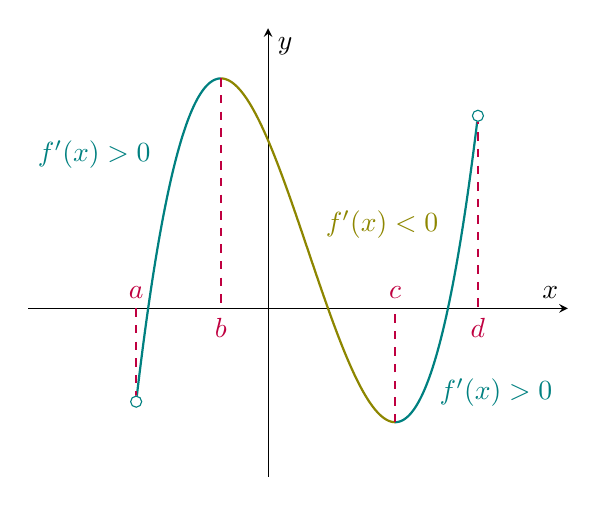
\begin{tikzpicture}
			\begin{axis}[
			axis lines = center, 
			xmin = -4, xmax = 5,
			ymax = 10,ymin = -6,
			ticks = none,
			xlabel = $x$, ylabel = $y$
			]
				\addplot[thick, color = teal, domain = -2.2:-0.7863, samples = 100] {x^3-2*x^2-5*x+6};
				\addplot[thick, color = olive, domain = -0.7863:2.1196, samples = 100] {x^3-2*x^2-5*x+6};
				\addplot[thick, color = teal, domain = 2.1196:3.5, samples = 100] {x^3-2*x^2-5*x+6};
				\draw[thick, dashed, color = purple] (axis cs: -2.2,0) -- (axis cs: -2.2,-3.328);
				\draw[thick, dashed, color = purple] (axis cs: -0.7863,8.2088) -- (axis cs: -0.7863,0);
				\draw[thick, dashed, color = purple] (axis cs: 2.1196,-4.0607) -- (axis cs: 2.1196,0);
				\draw[thick, dashed, color = purple] (axis cs: 3.5,6.875) -- (axis cs: 3.5,0);
				\node[anchor = south, color = purple] at (axis cs: -2.2,0) {$a$};
				\node[anchor = north, color = purple] at (axis cs: -0.7863,0) {$b$};
				\node[anchor = south, color = purple] at (axis cs: 2.1196,0) {$c$};
				\node[anchor = north, color = purple] at (axis cs: 3.5,0) {$d$};
				\filldraw[color = white] (axis cs: -2.2,-3.328) circle (2pt);
				\draw[color = teal] (axis cs: -2.2,-3.328) circle (2pt);
				\filldraw[color = white] (axis cs: 3.5,6.875) circle (2pt);
				\draw[color = teal] (axis cs: 3.5,6.875) circle (2pt);
				\node[color = teal, anchor = east] at (axis cs: -1.8,5.5) {$f'(x)>0$};
				\node[color = olive, anchor = west] at (axis cs: 0.8,3) {$f'(x)<0$};
				\node[color = teal, anchor = west] at (axis cs: 2.7,-3) {$f'(x)>0$};
			\end{axis}
		\end{tikzpicture}
		}
		\caption{Monotoniforhold for funktion $f$.}
		\label{fig:monotoniforhold}
		\end{minipage}
		\begin{minipage}{0.45\textwidth}
			\centering
			\resizebox{0.9\textwidth}{!}{
			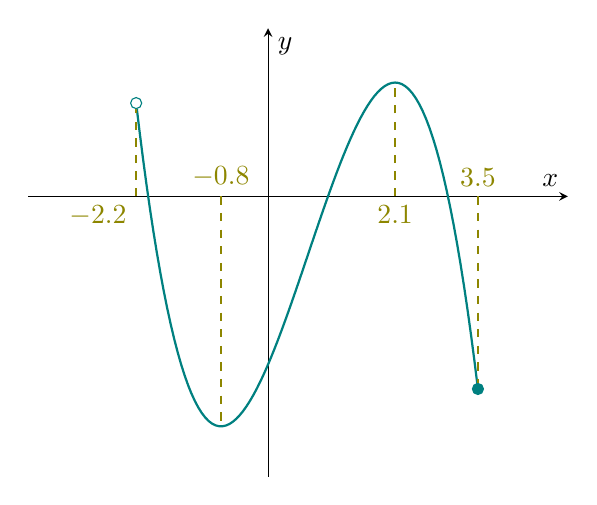
\begin{tikzpicture}
				\begin{axis}
				[ axis lines = center, 
				xmin = -4, xmax = 5,
				ymin =-10, ymax = 6,
				xlabel = $x$, ylabel = $y$,
				ticks = none, 
				]
					\addplot[color = teal, thick, samples = 100, domain = -2.2:3.5] {-x^3 + 2*x^2 + 5*x - 6};
					\draw[dashed, color = olive, thick] (axis cs: -2.2,0) -- (axis cs: -2.2,3.328);
					\draw[dashed, color = olive, thick] (axis cs: 3.5,0) -- (axis cs: 3.5,-6.875);
					\draw[dashed, color = olive, thick] (axis cs: 2.1196,0) -- (axis cs:2.1196,4.0607);
					\draw[dashed, color = olive, thick] (axis cs: -0.7863,0) -- (axis cs:-0.7863,-8.2088);
					\filldraw[color = white] (axis cs: -2.2, 3.328) circle (2pt);
					\draw[color = teal] (axis cs: -2.2, 3.328) circle (2pt);
					\filldraw[color = teal] (axis cs: 3.5,-6.875) circle (2pt);
					\node[color = olive, anchor = north east] at (axis cs: -2.2,0 ) {$-2.2$};
					\node[color = olive, anchor = south] at (axis cs: 3.5,0) {$3.5$};
					\node[color = olive, anchor = south] at (axis cs: -0.7863,0) {$-0.8$};
					\node[color = olive, anchor = north] at (axis cs: 2.1196,0) {$2.1$};
				\end{axis}
			\end{tikzpicture}
			}
			\caption{Aflæsning af monotoniforhold for funktion $g$.}
			\label{fig:monotonimedtal}
		\end{minipage}
	\end{figure}
	Betragter vi i stedet Figur \ref{fig:monotonimedtal} kan vi opskrive \textit{monotoniforholdene} for $g$.
	\begin{itemize}
		\item[$\cdot$] Funktionen $g$ er voksende for alle $x$ på intervallet $]-2.2,-0.8]$.
		\item[$\cdot$] Funktionen $g$ er aftagende for alle $x$ på intervallet $[-0.8,2.1]$.
		\item[$\cdot$] Funktionen $g$ er voksende for alle $x$ på intervallet $[2.1,3.5]$.
	\end{itemize}
	Bemærk, at intervalklammen i første interval $]-2.2,-0.8]$ vender væk fra tallet, da tallet ikke er en del 
	af definitionsmængden for $g$. Dette kan ses ved at punktet på Figur \ref{fig:monotonimedtal} er udhulet. 
\end{exa}
Vi kalder stederne, hvor funktioner skifter fra at være voksende til aftagende og vice versa for \textit{ekstrema}. Disse kan både være \textit{maksima} og \textit{minima}. Vi har følgende sætning, der siger noget om betingelserne for ekstrema
\begin{setn}[Ekstrema]
	Hvis $f'(x_0) = 0$, så har $f$ enten et lokalt maksimum, et lokalt minimum eller en 
	\textit{vandret vendetangent} i $x_0$. 
\end{setn}
\begin{figure}[H]
	\centering
	\begin{minipage}{0.3\textwidth}
		\centering
		\resizebox{0.9\textwidth}{!}{
		\begin{tikzpicture}
			\begin{axis}
			[
			axis lines = center, 
			xmin = -1, xmax = 3,
			ymin = -1, ymax = 2, 
			ticks = none,
			xlabel = $x$, ylabel = $y$
			]
				\addplot[color = teal, thick, samples = 100, domain = -1:3] {-x^2+2.5*x};
				\draw[dashed, color = olive, thick] (axis cs: 1.25,0) -- (axis cs: 1.25,25/16);
				\node[color = olive, anchor = north] at (axis cs: 1.25,0) {$x_0$};
			\end{axis}
		\end{tikzpicture}
		}
		\caption{Maksimum i $x_0$.}
		\label{fig:max}
	\end{minipage}
	\begin{minipage}{0.3\textwidth}
		\centering
		\resizebox{0.9\textwidth}{!}{
		\begin{tikzpicture}
			\begin{axis}
			[
			axis lines = center, 
			xmin = -1, xmax = 3,
			ymin = -2, ymax = 1, 
			ticks = none,
			xlabel = $x$, ylabel = $y$
			]
				\addplot[color = teal, thick, samples = 100, domain = -1:3] {x^2+-2.5*x};
				\draw[dashed, color = olive, thick] (axis cs: 1.25,0) -- (axis cs: 1.25,-25/16);
				\node[color = olive, anchor = south] at (axis cs: 1.25,0) {$x_0$};
			\end{axis}
		\end{tikzpicture}
		}
		\caption{Minimum i $x_0$.}
	\end{minipage}
	\begin{minipage}{0.3\textwidth}
		\centering
		\resizebox{0.9\textwidth}{!}{
		\begin{tikzpicture}
			\begin{axis}
			[
			axis lines = center, 
			xmin = -1, xmax = 3,
			ymin = -1, ymax = 2, 
			ticks = none,
			xlabel = $x$, ylabel = $y$
			]
				\addplot[color = teal, thick, samples = 100, domain = -1:3] {(x-1)^3 + 1};
				\draw[dashed, color = olive, thick] (axis cs: 1,0) -- (axis cs: 1,1);
				\node[color = olive, anchor = north] at (axis cs: 1,0) {$x_0$};
			\end{axis}
		\end{tikzpicture}
		}
		\caption{Vendetangent i $x_0$.}
	\end{minipage}
\end{figure}

\begin{exa}
	Funktionen $g$, der fremgår af Figur \ref{fig:monotonimedtal} har et minimum i $x = -0.8$. Dette er desuden
	et \textit{globalt minimum}, da der ikke er andre værdier for $x$, der giver $g$ en mindre funktionsværdi.
	$g$ har desuden et globalt maksimum i $x = 2.1$. 
\end{exa}
\begin{exa}
	Vi kan ikke se hele definitionsmængden for grafen på Figur \ref{fig:max}. Vi antager, at det er en parabel. I dette tilfælde vil monotoniforholdene lyde:
	\begin{itemize}
		\item[$\cdot$] Funktionen $f$ er voksende på intervallet $]-\infty,x_0]$.
		\item[$\cdot$] Funktionen $f$ er aftagende på intervallet $[x_0,+\infty[$.
	\end{itemize}
\end{exa}
\newpage

\subsection*{Opgave 1}	

Følgende er grafen for polynomiet $f$ givet ved
\begin{align*}
	f(x) = x^2.
\end{align*}
\begin{center}
	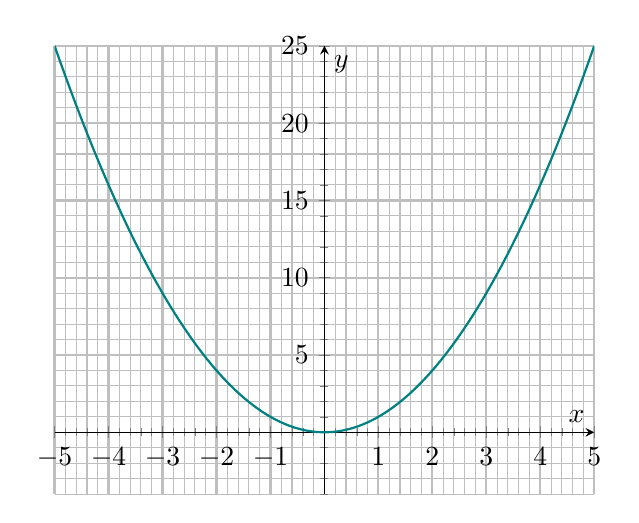
\begin{tikzpicture}
		\begin{axis}
		[
		axis lines = center, 
		xmin = -5, xmax = 5,
		ymin = -4, ymax = 25, 
		xlabel = $x$, ylabel = $y$,
		xtick = {-5,-4,...,4,5},
		grid = both, minor tick num = 4,
		major grid style = {line width = 0.8pt}
		]
			\addplot[color = teal, thick, samples = 100, domain = -5:5] {x^2};
		\end{axis}
	\end{tikzpicture}
\end{center}
\begin{enumerate}[label=\roman*)]
	\item Bestem hældningen af tangenten gennem punktet $(1,f(1))$ ved brug af en lineal. 
	\item Bestem en ligning på formen $y = ax + b$ for tangenten gennem dette punkt. 
	\item For hvilke værdier af $x$ er $f'(x) > 0?$ 
	\item Bestem differentialkvotienten i punkterne $(-4,f(-4))$, $(-3,f(-3))$ osv. frem til $(5,f(5))$.
	\item Kan du gennemskue en formel til at bestemme differentialkvotient for $f$, hvis $f(x) = x^2$?
\end{enumerate}

\newpage
\subsection*{Opgave 2}

Følgende er grafen for polynomiet $f$ givet ved
\begin{align*}
	f(x) = x^3.
\end{align*}
\begin{center}
	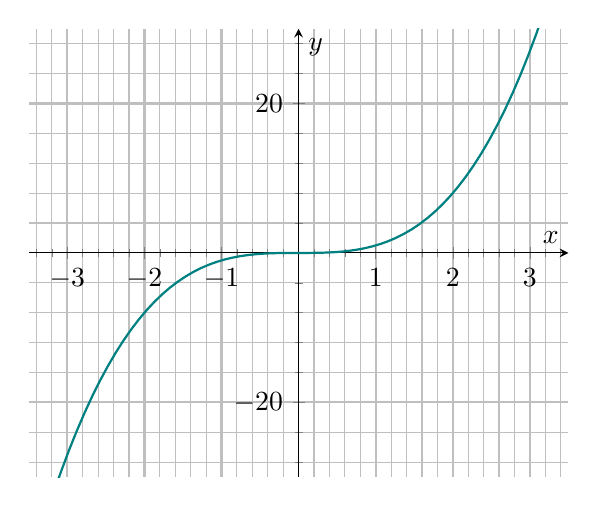
\begin{tikzpicture}
		\begin{axis}
		[
		axis lines = center, 
		xmin = -3.5, xmax = 3.5,
		ymin = -30, ymax = 30, 
		xlabel = $x$, ylabel = $y$,
		xtick = {-5,-4,...,4,5},
		grid = both, minor tick num = 4,
		major grid style = {line width = 0.8pt}
		]
			\addplot[color = teal, thick, samples = 100, domain = -5:5] {x^3};
		\end{axis}
	\end{tikzpicture}
\end{center}
	
\begin{enumerate}[label=\roman*)]
	\item Bestem hældningen af tangenten gennem punktet $(-2,f(-2))$ ved brug af en lineal. 
	\item Bestem $f'(x_0)$ for $x=-3,-2,-1,0,1,2,3$ ved brug af lineal
	\item Kan du gennemskue en formel til at bestemme $f'$, hvis $f(x) = x^3$?
	\item Hvad ville formlen for $f'$ være, hvis $f(x) = x^4$?
	\item Hvad ville formlen for $f'$ være, hvis $f(x) = x^n$?
\end{enumerate}

\newpage
\subsection*{Opgave 3}
Følgende er grafen for en funktion $f$.
\begin{center}
	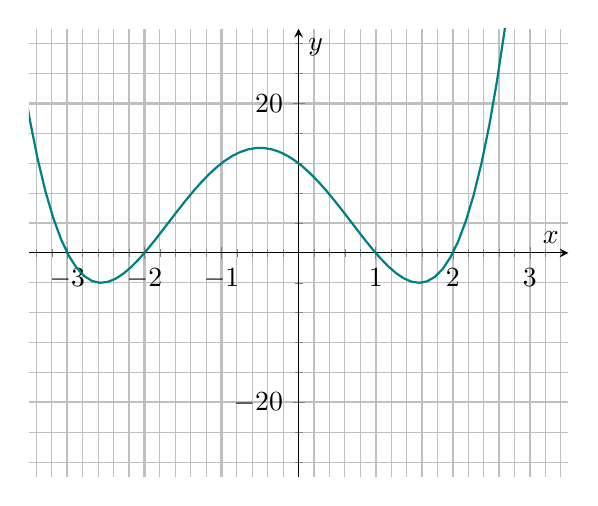
\begin{tikzpicture}
		\begin{axis}
		[
		axis lines = center, 
		xmin = -3.5, xmax = 3.5,
		ymin = -30, ymax = 30, 
		xlabel = $x$, ylabel = $y$,
		xtick = {-5,-4,...,4,5},
		grid = both, minor tick num = 4,
		major grid style = {line width = 0.8pt}
		]
			\addplot[color = teal, thick, samples = 100, domain = -5:5] {(x-2)*(x-1)*(x+2)*(x+3)};
		\end{axis}
	\end{tikzpicture}
\end{center}
\begin{enumerate}[label=\roman*)]
	\item Bestem $f'(-3)$, $f'(-0.5), f'(1)$ og $f'(2.2)$.
	\item Hvor har $f$ ekstrema og hvilke typer af ekstrema er det?
	\item Bestem differentialkvotienten i ekstremaerne for $f$.
	\item Opskriv monotoniforholdene for $f$. 
\end{enumerate}

\newpage
\subsection*{Opgave 4}
Grafen for en funktion $f$ er givet:

\begin{center}
	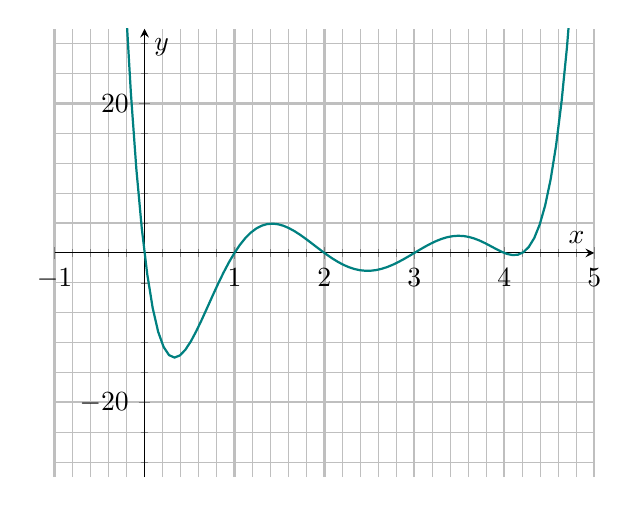
\begin{tikzpicture}
		\begin{axis}
		[
		axis lines = center, 
		xmin = -1, xmax = 5,
		ymin = -30, ymax = 30, 
		xlabel = $x$, ylabel = $y$,
		xtick = {-5,-4,...,4,5},
		grid = both, minor tick num = 4,
		major grid style = {line width = 0.8pt}
		]
			\addplot[color = teal, thick, samples = 100, domain = -1:5] {(x)*(x-1)*(x-2)*(x-3)*(x-4)*(x-4.2)};
		\end{axis}
	\end{tikzpicture}
\end{center}

\begin{enumerate}[label=\roman*)]
	\item Bestem ekstrema for $f$ og afgør, hvilken type ekstrema, de er. 
	\item Bestem monotoniforholdene for $f$.
\end{enumerate}
	